\section{Independent nuisance information and the variational form}
\label{sec:prior}

Preparation measurements, calibration data, or external control information can constrain nuisance coefficients. Let $\Lambda\succeq0$ denote the corresponding independent local precision matrix. The combined Fisher block is
\begin{equation}
F_\Lambda=\begin{pmatrix}
\bm s^T\bm s & \bm s^T J\\
J^T\bm s & J^T J+\Lambda
\end{pmatrix},
\end{equation}
and the profiled target information is
\begin{equation}
 \Iprior=\bm s^T\bm s-
 \bm s^T J(J^TJ+\Lambda)^+J^T\bm s.
\label{eq:priorfisher}
\end{equation}

\paragraph*{Proposition 4 (variational profiling identity).}
For $\Lambda\succeq0$,
\begin{equation}
 \boxed{\displaystyle
 \Iprior=\min_{\bm a\in\mathbb R^m}
 \left[\|\bm s-J\bm a\|_2^2+\bm a^T\Lambda\bm a\right].}
\label{eq:variational}
\end{equation}

\emph{Proof.} Expand the objective as
\begin{equation}
 \bm s^T\bm s-2\bm a^TJ^T\bm s
 +\bm a^T(J^TJ+\Lambda)\bm a.
\end{equation}
For every $z\in\Null(J^TJ+\Lambda)$, positivity of both terms implies $Jz=0$ and $\Lambda^{1/2}z=0$, hence $z^TJ^T\bm s=0$. Thus $J^T\bm s$ belongs to the range of $J^TJ+\Lambda$ and the minimum is attained by the pseudoinverse solution. Substitution gives Eq.~\eqref{eq:priorfisher}. \hfill$\square$

Two corollaries are immediate.

\paragraph*{Corollary 4.1 (nuisance-coordinate invariance).}
For any invertible nuisance transformation $\bm a=M\bm\phi$,
\begin{equation}
 J_\phi=JM,\qquad \Lambda_\phi=M^T\Lambda M,
\end{equation}
and $\mathcal I_\beta$ is unchanged. This follows because Eq.~\eqref{eq:variational} is the same minimization written in bijectively related coordinates.

\paragraph*{Corollary 4.2 (calibration-information monotonicity).}
If $\Lambda_2-\Lambda_1\succeq0$, then
\begin{equation}
 \mathcal I_\beta(\Lambda_2)\ge\mathcal I_\beta(\Lambda_1).
\label{eq:priormono}
\end{equation}
For every trial nuisance coefficient, the objective in Eq.~\eqref{eq:variational} can only increase when a positive-semidefinite penalty is added; therefore its minimum cannot decrease.

The language here requires care. If $\bm s\in\Col(J)$, the target is not structurally identifiable from the detector data alone at first order, even if $\mathcal I_\beta(\Lambda)>0$ after external nuisance information is added. The latter is \emph{prior-assisted or calibration-assisted precision}, not data-only identification. This distinction prevents an external constraint from being misreported as information created by the science channel.

\subsection{Exact amplitude obstruction and prior rescue}

The minimal RQIR reference model takes
\begin{equation}
 \bm s_0=(1,0)^T,\qquad J=\bm s_0.
\end{equation}
The science and nuisance scores are exactly aligned, so $\mathcal I_\beta(0)=0$. If an independent preparation measurement contributes scalar precision $C_a$, Eq.~\eqref{eq:priorfisher} gives
\begin{equation}
 \boxed{\displaystyle
 \mathcal I_\beta(C_a)=\frac{C_a}{1+C_a}.}
\label{eq:priorrescue}
\end{equation}
The RQIR-STAT-001 certificate checks $C_a=1,4,9,19,99$, giving $0.5,0.8,0.9,0.95,0.99$, respectively.

\begin{figure}[t]
\centering
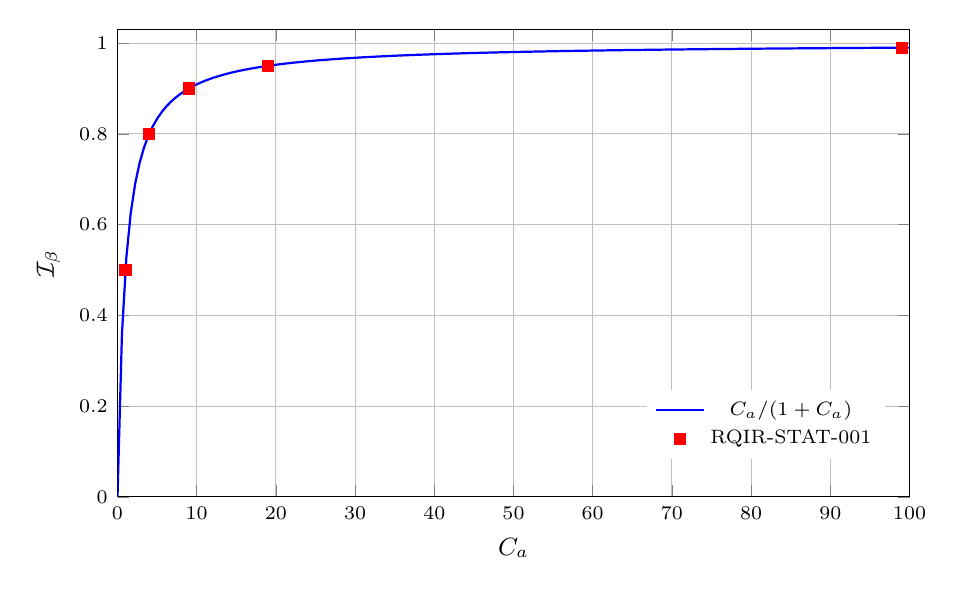
\begin{tikzpicture}
\begin{axis}[
 width=0.96\columnwidth,height=0.62\columnwidth,
 xlabel={$C_a$},ylabel={$\mathcal I_\beta$},
 xmin=0,xmax=100,ymin=0,ymax=1.03,
 grid=major,legend style={font=\scriptsize,draw=none,at={(0.97,0.08)},anchor=south east},
 tick label style={font=\scriptsize},label style={font=\small}]
\addplot[blue,thick,domain=0:100,samples=180] {x/(1+x)};
\addlegendentry{$C_a/(1+C_a)$}
\addplot[only marks,mark=square*,red] coordinates {(1,0.5) (4,0.8) (9,0.9) (19,0.95) (99,0.99)};
\addlegendentry{RQIR-STAT-001}
\end{axis}
\end{tikzpicture}

\caption{Calibration-assisted recovery for the exactly aligned amplitude model, Eq.~\eqref{eq:priorrescue}. The curve approaches the unit raw Fisher but never changes the fact that the detector data alone have zero first-order information at $C_a=0$. Markers are deterministic RQIR-STAT-001 points. Plotting code was AI-assisted; values were checked by a separate deterministic audit script against the analytic formula.}
\label{fig:priorrescue}
\end{figure}

